\chapter{Invisible width measurement}
\label{chap:inv-width-extraction}

%\chapterquote{}{}

\section{Introduction}

The key ingredients into extracting the \PZ invisible width from Eq.~\ref{eq:zinv} includes the \IZvvj and \IZllj processes. These are estimated from the \metplusjets and \diellplusjets region with background subtraction through data driven methods or MC estimation. The comparison of the predictions to data for these regions are presented in this chapter, acting as the input for the likelihood fit. The details of the likelihood fit are discussed along with the results of the fit in terms of the nuisance parameters, their impact on the parameter of interest itself, the \PZ invisible width.


\section{Signal regions}

The SM prediction for the \IZvvj and \IZllj processes from MC simulations
predict the rate of events by estimating the efficiency and acceptance of the
selection applied, with data-driven corrections where relevant. The
normalisation on these processes is estimated from a likelihood fit to that
data, exploiting the shape of the \recoil distribution. The shapes of each
process is taken from MC, with the associated uncertainties affecting the
normalisation and morphing the shapes, within their gaussian constraints.


\subsection{\diellplusjets region}

The selection applied to the \diellplusjets is designed for similar kinematics
between the signal processes. This is primarily achieved through the \recoil
parameter which is well modelled in MC, as shown in
Sec.~\ref{sec:ptmiss-calib}. Furthermore, the selections differ by kinematic
requirements on the final state leptons, including their \pt and invariant
mass. These kinematic distributions are shown for the \dimuplusjets and
\dieleplusjets regions in Fig.~\ref{fig:doublemuon-dists} and
\ref{fig:doubleelectron-dists}, respectively.
%
\begin{figure}[htb]
    \centering
    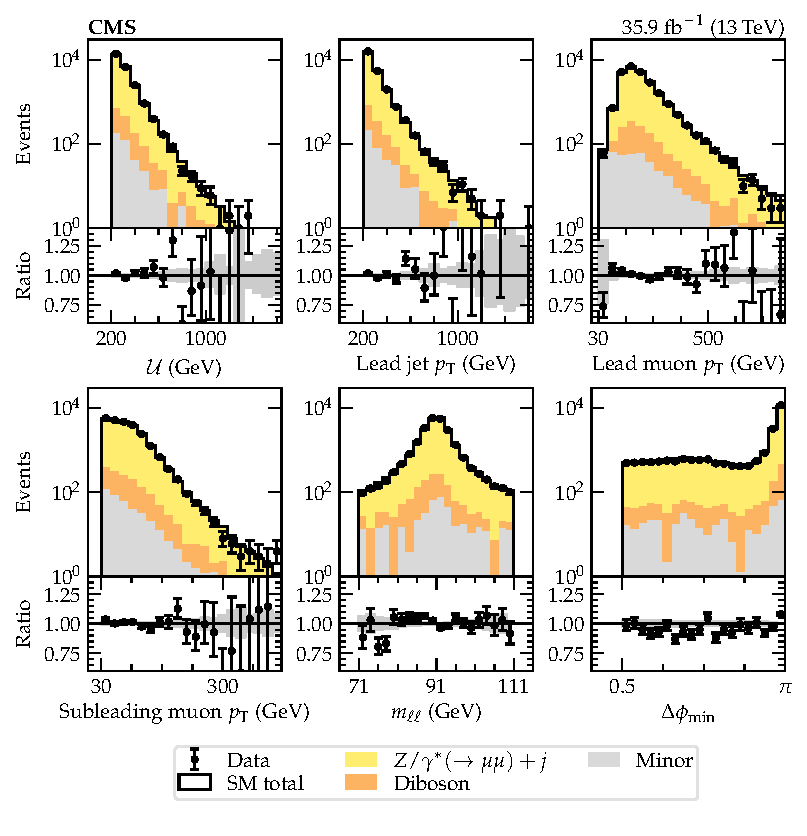
\includegraphics{chapters/043_results/images/doublemuon_dists.pdf}
    \caption[Dimuon kinematics.]{
        Kinematic distributions within the \dimuplusjets region. The ratio is taken with respect to the SM total prediction and includes the MC statistical uncertainties, whereas systematic uncertainties have been omitted.
    }
    \label{fig:doublemuon-dists}
\end{figure}
%
\begin{figure}[htb]
    \centering
    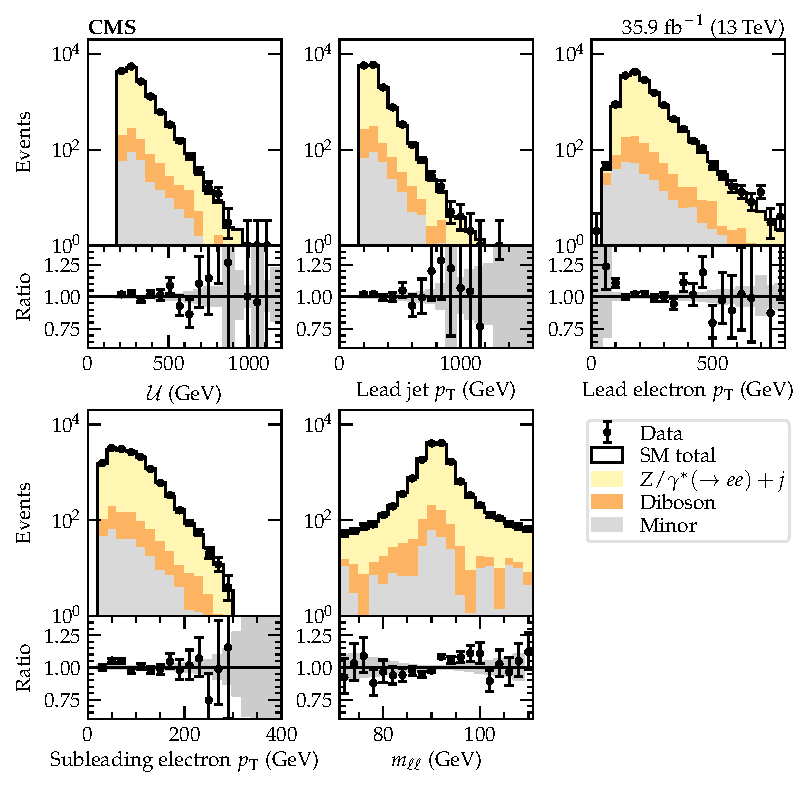
\includegraphics{chapters/043_results/images/doubleelectron_dists.pdf}
    \caption[Dielectron kinematics.]{
        Kinematic distributions within the \dieleplusjets region, equivalent to those shown in Fig.~\ref{fig:doublemuon-dists}.
    }
    \label{fig:doubleelectron-dists}
\end{figure}
%
Both regions are enriched in the \IDYllj process ($94\%$), with the largest
background from diboson production ($4$--$5\%$) and a smaller contribution
from other minor backgrounds ($1$--$2\%$). These backgrounds are determined
from NLO MC, without any additional data-driven correction. The systematic
uncertainties associated with these processes are included in the background
subtraction performed within the likelihood fit. The data and MC distributions
are within agreement, both for their shape and normalisations, with slight
deviations in the invariant mass distribution, covered by systematic
uncertainties in the lepton $\pt$. The requirement placed on the recoil and lead jet \pt
result in the sculpting of the lead and subleading muon
distributions, while the invariant mass window is centred on the \PZ mass.


\subsection{\metplusjets region}

The \metplusjets region consists primarily of the \IZvvj process ($59.1\%$)
with a significant background from \IWlvj ($34.6\%$) and minor contributions
from $t$-quark production ($1.7\%$), QCD multijet ($0.7\%$) and other
processes ($3.9\%$). The \IWlvj process is modified by the data-driven
estimate through the transfer factor approach. Similarly, the QCD multijet
contribution includes a data-driven estimate from an extrapolation from the
QCD multijet enriched sidebands. The other backgrounds are estimated from NLO
MC predictions. The kinematic distributions for the \metplusjets region,
without the data-driven estimates, are shown in Fig.~\ref{fig:monojet-dists}.
%
\begin{figure}[htb]
    \centering
    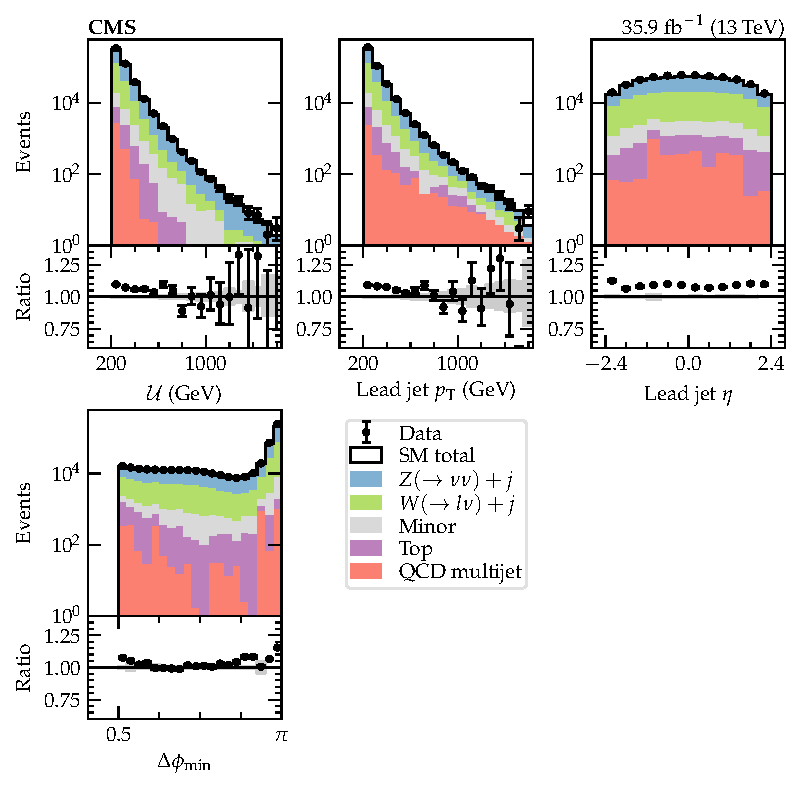
\includegraphics{chapters/043_results/images/monojet_dists.pdf}
    \caption[\metplusjets kinematics.]{
        Kinematic distributions within the \metplusjets region, similar to those shown in Fig.~\ref{fig:doublemuon-dists}.
    }
    \label{fig:monojet-dists}
\end{figure}
%
The data and SM prediction distributions disagree, however, the large \IWlvj contribution has a $10\%$ correction determined from the data-driven transfer factors. The correction covers the discrepancy seen between data and the SM prediction.


\section{Likelihood fit}

The \PZ invisible width is estimated from a simultaneous fit to the data
between the \metplusjets, \diellplusjets and \ellplusjets ($\ell=e,\mu$)
regions under the likelihood formalism (App.~\ref{app:likelihood}). The \IWj
estimation through the transfer factor approach is implemented by a global
unconstrained parameter which scales the \IWj process in the \metplusjets and
\ellplusjets. Such a parameter is constrained by the data in the \IWj enriched
control regions and applied to the same process in the \metplusjets region,
improving the accuracy of the prediction along with correcting normalisation
issues. To extract the invisible width, the \IZllj process is scaled by a
parameter $r_\PZ$ while \IZvvj is scaled by $r_\PZ r_{\inv}$. The observed
number of events for a particular process may be expressed as the product of
the cross section, branching fraction, analysis efficiency and acceptance.
Setting $r_\inv=r_\PZ=1$ corresponds to the SM expected number of events for
the process. Therefore, taking the ratio of Eq.~\ref{eq:zinv} with its SM
expectation gives
%
\begin{equation}
    r_\inv = \frac{\Gamma(\PZ\ra\inv)}{\Gamma_{\mathrm{SM}}(\PZ\ra\inv)}\ ,
\end{equation}
%
where $\Gamma_{\mathrm{SM}}$ corresponds to the SM expected width.

The postfit distributions from the simultaneous fit are shown in Fig.~\ref{fig:finalfit-postfit}
%
\begin{figure}
    \centering
    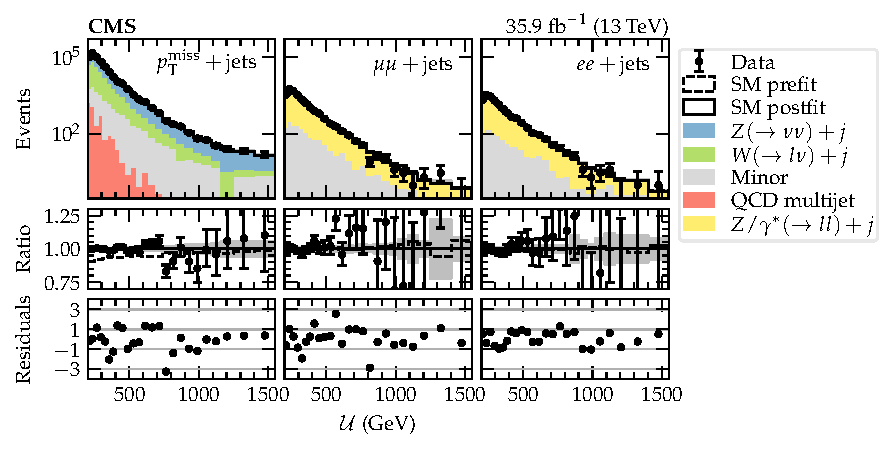
\includegraphics{chapters/043_results/images/finalfit-postfit.pdf}
    \caption[Recoil distributions after a fit to the data between the signal and control regions.]{
        \recoil distributions for the signal regions to determine the rate of \IZvvj and \IZllj. The ratio is taken with respect to the SM postfit and includes the prefit result to show the effect of including the scaling factors. The residuals display the difference between the data and the SM postfit results, normalised by their uncertainties summed in quadrature.
    }
    \label{fig:finalfit-postfit}
\end{figure}
%
A significant improvement with the postfit results in the \ptmissplusjets
region compared to the prefit as a result of the data-driven scaling parameter
of $10\%$ determined for the \IWlvj process. The QCD multijet process is
corrected by up to a factor of $3$ in the tail of the \recoil distribution.
However, this process remains to be a small background. There is no
significant difference between the postfit and prefit results in the
\diellplusjets regions. Furthermore, one data point is beyond the $3\sigma$
band of the postfit result, however, since there are $75$ bins here, along
with another $50$ in the \ellplusjets regions, this is not a concern and falls
within standard expectations. The associated postfit nuisance parameters and
their impact on the $r_{\mathrm{inv}}$ parameter is shown in
Fig.~\ref{fig:finalfit-impacts}.
%
\begin{figure}
    \centering
    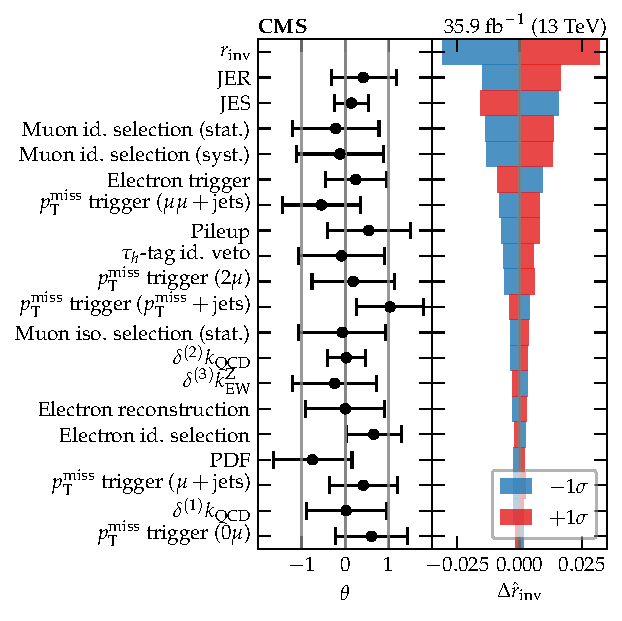
\includegraphics{chapters/043_results/images/finalfit-impacts.pdf}
    \caption[Nuisance parameters after a fit to the data between the signal and control regions.]{
        Nuisance parameter ($\theta$) pulls, constraints and impacts on $r_{\mathrm{inv}}$ ($\Delta \hat{r}_{\mathrm{inv}}$). Only the 20 most impacting parameters are displayed.
    }
    \label{fig:finalfit-impacts}
\end{figure}
%
The postfit nuisance parameters are all within the $|\theta|<1$ level, with
constraints to a varying degree. The constraints on the jet energy resolution
(JER) and scale (JES) are consistent with the results found for the \ptmiss
scale and resolution (Sec.~\ref{sec:ptmiss-calib}. Here, the uncertainties
were dominated by the jet energy corrections and consistently over-covered the
data from the parallel components which plays the largest role in the \recoil
distribution. The nuisance parameter $\delta^{(2)}k_{\mathrm{QCD}}$ is
associated with a possible shape dependence with the \recoil distribution from
the choice of factorisation and renormalisation scale. However, this has a
partial double-counting with the $\delta^{(1)}k_{\mathrm{QCD}}$ parameter
which probes the normalisation variation from the choice of these scales.
Otherwise, no other nuisance parameters are significantly constrained. Among
the JER and JES uncertainties, the muon identification selection, electron and
\ptmiss trigger have the largest impact on the $r_{\mathrm{inv}}$ parameter.
These are expected considering the final states associated with the regions
probed.

The multi-dimensional minimisation of the likelihood may be profiled onto a
single dimension by remaining within the minimum for various fixed values of
the dimension of interest. The value of the minimum is subtracted from
subsequent likelihood profile values to give $-2\Delta\log L$, where the
confidence interval in terms of the number of standard deviations $n_{\sig}$
is given by the intersection points of $-2\Delta\log L=n_{\mathrm{sig}}^2$.
The profile for the $r_{\mathrm{inv}}$ is shown in
Fig.~\ref{fig:finalfit-scan-1d}.
%
\begin{figure}
    \centering
    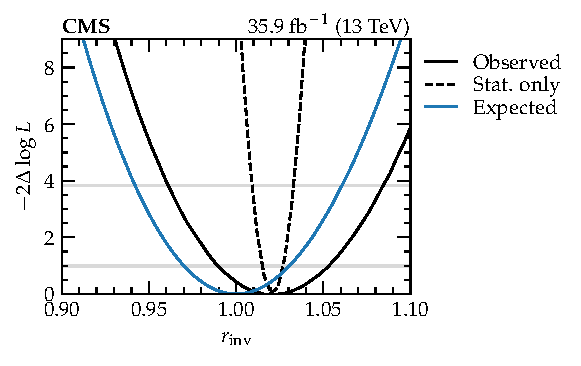
\includegraphics{chapters/043_results/images/finalfit-scan-1d.pdf}
    \caption[Likelihood profile in the $r_{\mathrm{inv}}$ dimension.]{
     Likelihood profile across the $r_{\mathrm{inv}}$ dimension for the fit to data (observed) and an alternative fit where the data is set to the prediction in the poisson terms of the likelihood (expected). This is typically known as the Asimov dataset and gives the expected results with all the parameters set to their input values. In addition, a fit to the data with the systematic uncertainties fixed at their postfit values (stat. only) is included to compare the effect of statistical and systematic uncertainties. The measurement of the $r_{\mathrm{inv}}$ parameter is systematically limited.
    }
    \label{fig:finalfit-scan-1d}
\end{figure}
%
It is also instructive to perform the scan in 2-dimensions with a modified fit
where the \IZvvj and \IZllj processes are scaled by separate parameters,
$r_{\mathrm{inv}}$ and $r_{\ell\ell}$ respectively. This 2-dimensional scan is
shown in Fig.~\ref{fig:finalfit-scan-2d}, showing that the measurement is consistent with the SM prediction.
%
\begin{figure}
    \centering
    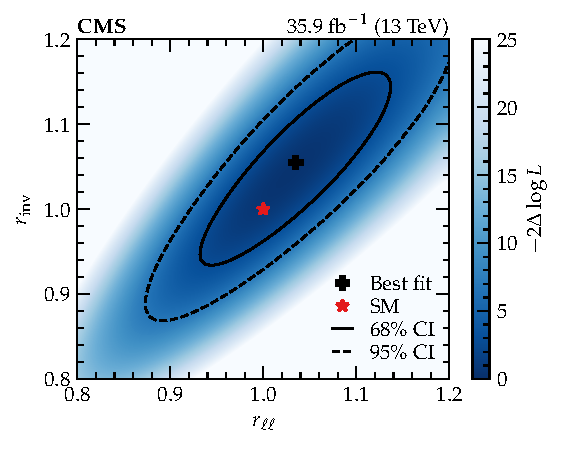
\includegraphics{chapters/043_results/images/finalfit-scan-2d.pdf}
    \caption[Two-dimensional likelihood profile in the $r_{\mathrm{inv}}$--$r_{\ell\ell}$ plane.]{
        Two-dimensional likelihood profile in the $r_{\mathrm{inv}}$--$r_{\ell\ell}$ plane for a fit with uncorrelated scaling parameters on the \IZvvj and \IZllj processes. The SM prediction is within the $68\%$ confidence interval (CI) with the best fit point slightly higher in both parameters. The nominal fit with the single parameter of interest $r_{\mathrm{inv}}$ can be interpreted as the gradient of the line through the origin to any point on the plane. Therefore, the uncertainty associated with this parameter is less than the uncertainty of the separate parameters.
    }
    \label{fig:finalfit-scan-2d}
\end{figure}
%

The best fit value of the parameter of interest and its associated uncertainty is measured as
%
\begin{equation}
    r_{\mathrm{inv}} = 1.021\pm 0.006\ (\mathrm{stat.})\ \pm 0.031\ (\mathrm{syst.})\ .
\end{equation}
%
As with the likelihood profiles, this is consistent with the SM value of one, and is systematically dominated. This is translated into an invisible width, by scaling the SM prediction \cite{PhysRevD.98.030001},
%
\begin{equation}
    \Gamma_{\mathrm{inv}} = 512 \pm 3\ (\mathrm{stat.})\ \pm 16\ (\mathrm{syst.})\ \mathrm{MeV}\ ,
\end{equation}
%
with the summary of the direct measurement of the invisible width shown in Fig.~\ref{fig:finalfit-zinv}.
%
\begin{figure}
    \centering
    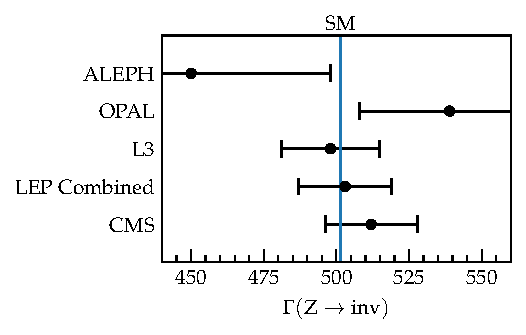
\includegraphics{chapters/043_results/images/finalfit-zinv.pdf}
    \caption[Summary of the invisible width measurements.]{
        Measurement of the \PZ invisible width by the LEP experiments and the result with the CMS experiment presented here. The SM prediction is included with a negligible uncertainty.
    }
    \label{fig:finalfit-zinv}
\end{figure}
%
The measurement presented is comparable to the LEP combined direct measurement.